\documentclass[main.tex]{subfiles}

%\externalcitedocument{bibfile}

\begin{document}

\chapter{IceCube Upgrade}\label{chapter:degg}

The IceCube Upgrade~\cite{ishihara2019icecube} is a planned expansion of the IceCube array designed to improve its sensitivity to low-energy neutrino events, which at the moment has a planned deployment for the 2025/6 south-pole season.
It will consist of seven additional strings of 700 optical sensors, which will be embedded near the bottom-center of the existing IceCube array where the ice is optically cleanest. 
An illustration of the Upgrade is shown in Figure~\ref{fig:upgrade_layout}
Two new optical sensors will be installed in Upgrade: the Multi-PMT Digital Optical Module (mDOM)~\cite{classen2019multipmt}, and the Ellipsoid Glass for Gen2 (D-Egg) module~\cite{degg}. 


\begin{figure}
    \centering
    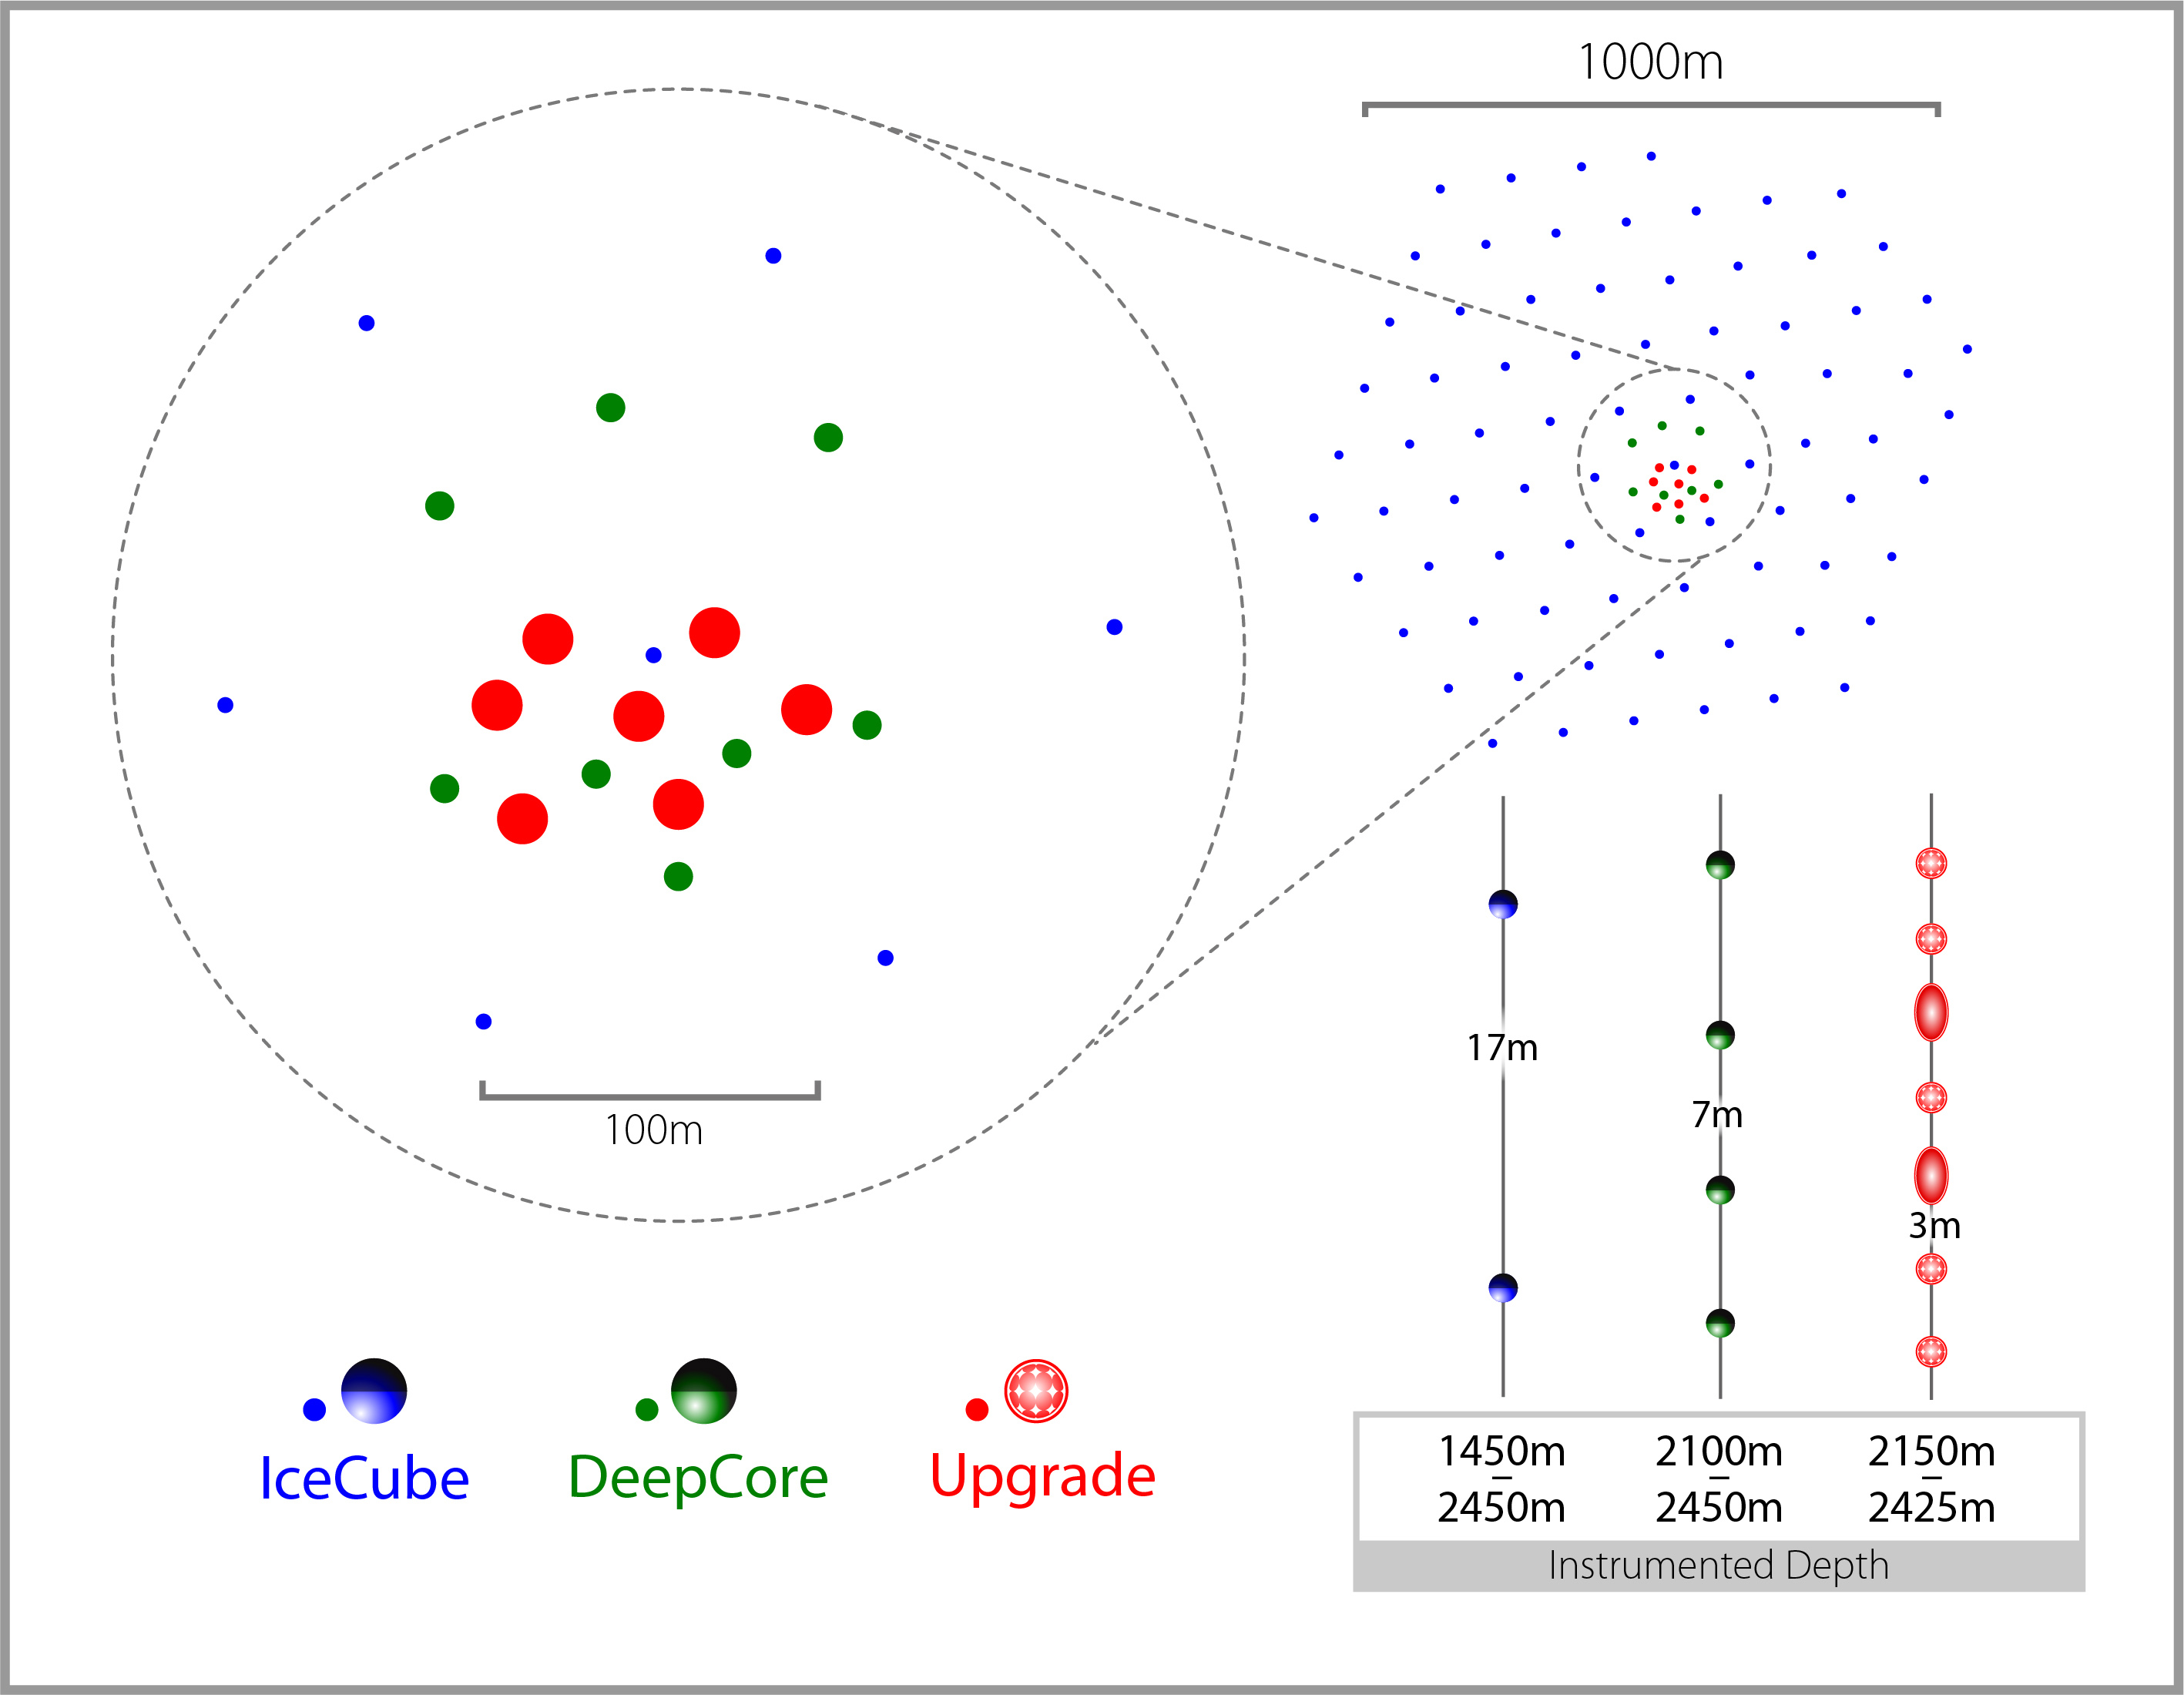
\includegraphics[width=0.7\linewidth]{figures/ICUpgradeLayout_V4b.jpg}
    \caption{A top-down view of the planned installation locations of IceCube Upgrade strings relative to existing IceCube and DeepCore strings.}
    \label{fig:upgrade_layout}
\end{figure}

These modules are designed to improve the photon detector efficiency and overall calibration of the detector within a small two megaton volume within the greater array. 
This will allow for the use of the main IceCube array to act as a veto layer for high-precision measurements of neutrino interactions in the $\mathcal{O}(1\sim 10\text{GeV})$ energy range. 
This will allow for the measurement of tau neutrino appearances with high precision, allow for cutting-edge measurements of neutrino oscillations, and to probe the unitarity of the Pontecorvo-Maki-Nakagawa-Sakata neutrino mixing matrix. 
Figure\ref{fig:tau_constrain_upgrade}, from Reference~\cite{ishihara2019icecube}, shows how well IceCube Upgrade will be able to constraint three-neutrino oscillations using only three years of data. 

\begin{figure}
    \centering
    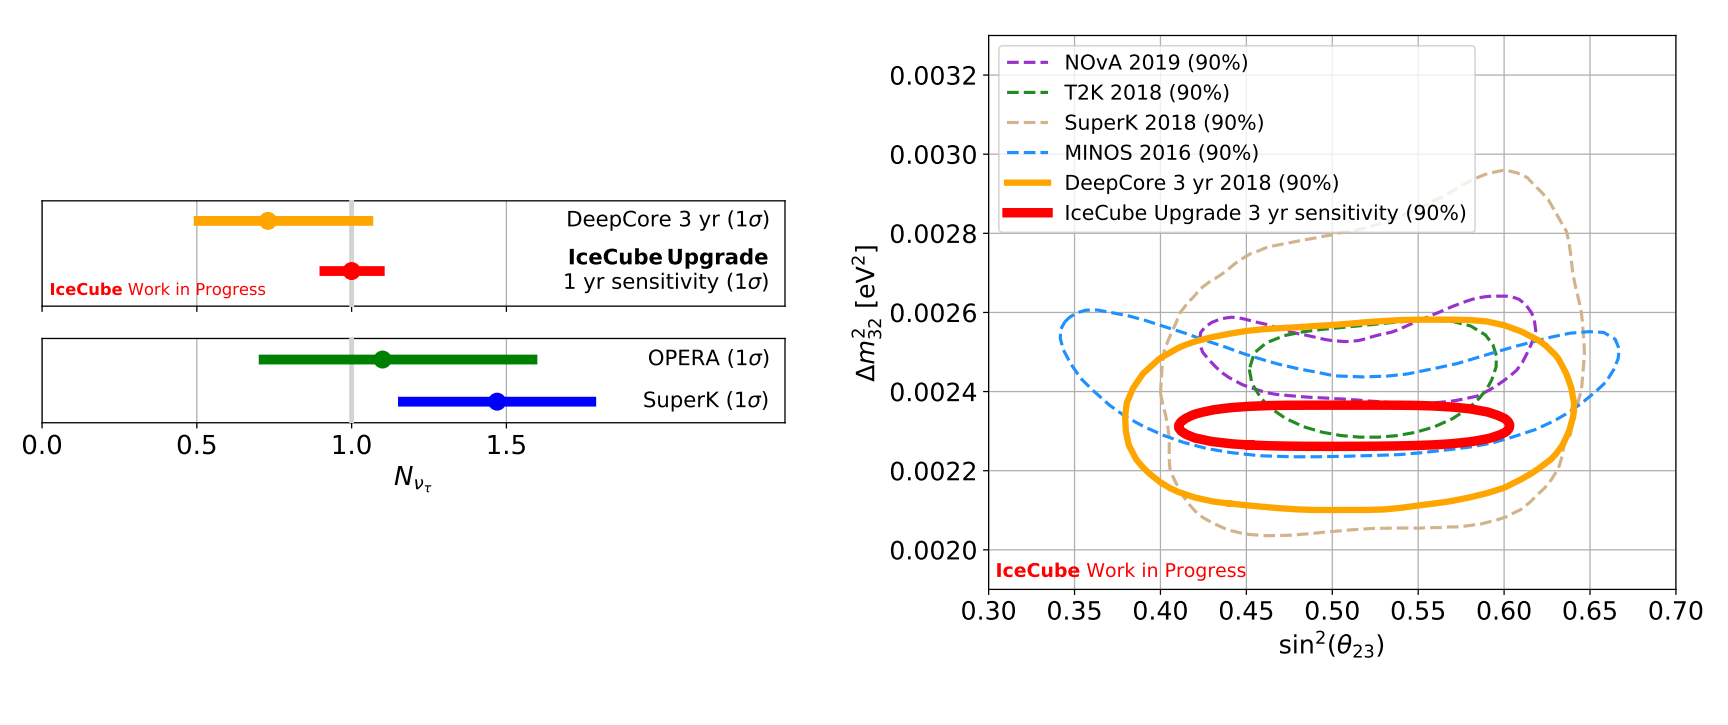
\includegraphics[width=0.85\linewidth]{figures/upgrade_physics.png}
    \caption{On the left, the $1\sigma$ sensitivity of the IceCube Upgrade (and other experiments) to constrain the normalization of the tau normalization, where we assume a normalization of one with one year of data. On the right, the predicted sensitivity of IceCube Upgrade to the 3$\nu$ oscillations parameters $\sin^{2}(\theta_{24})$ and $\Delta m_{32}^{2}$ with comparisons to References~\cite{PhysRevLett.120.071801, PhysRevD.98.052006, PhysRevLett.120.211801, WHITEHEAD2016130,Haegel_2017}}\label{fig:tau_constrain_upgrade}
\end{figure}


\section{IceCube D-Eggs}

The ``\textbf{D}ual optical sensors in an \textbf{E}llipsoid \textbf{G}lass for \textbf{G}en2,'' or D-Egg, is a new module designed for future extensions of IceCube. 
A schematic of a D-Egg is shown in Figure~\ref{fig:degg}
In particular, it is one of the planned optical modules to be deployed at the IceCube Neutrino Observatory as part of IceCube Upgrade, with a planned deployment in the 2025-2026 South Pole season.
The D-Eggs have been designed with an elongated egg-like shape and narrow cross-section to maximize its photon-sensitive area while maintaining a slim shape to reduce the time needed for deployment-hole drilling in the Antarctic ice to depths of up to 2,700 meters. 
Two 8-inch R5912-100-70 high-efficiency PMTs from Hamamatsu are used per D-Egg: one each facing upwards and downwards. 
Rather than the mu-metal cage, D-Eggs have a newer magnetic shielding made of FINEMET foil wrapped into a conical shape around the neck of each PMT.

In order to minimize damage to the sensitive PMTs, whenever a D-Egg is not actively being tested it is either kept in its shipping boxes or covered under a protective UV-opaque black plastic bag, as shown in Figure~\ref{fig:degg_bag}.

\begin{figure}
    \centering
    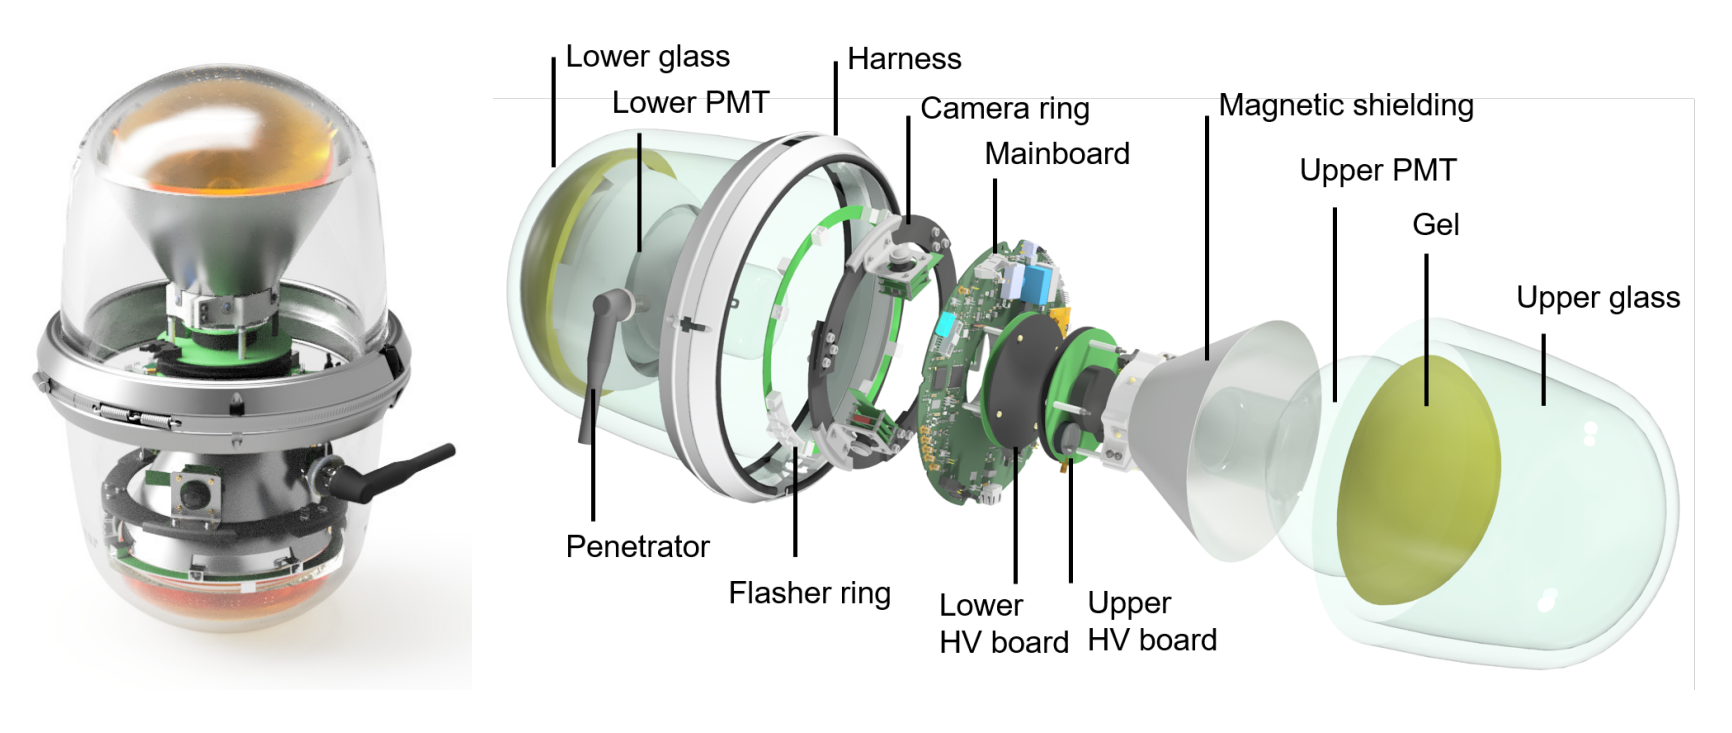
\includegraphics[width=\linewidth]{figures/degg.png}
    \caption{(left) A D-Egg with the harness around its equator, which is used to hold the device during deployment, and its sealed UV-transparent glass housing. (right) An exploded figuring showing the D-Egg internal structure, including: the mainboard, three cameras, twelve LED flashers, two PMTs, optical coupling silicone gel, and the magnetic shielding.}\label{fig:degg}
\end{figure}

\begin{figure}
    \centering
    \includegraphics[width=0.7\linewidth]{figures/degg/20221205011329_IMG_5420.JPG}
    \caption{A D-Egg PMT}
\end{figure}

\begin{figure}
    \centering
    \includegraphics[width=0.8\linewidth]{figures/degg/20221205005511_IMG_5401.JPG}
    \caption{Several D-Eggs are placed on carts and covered with opaque, protective, black plastic bags at an undisclosed location.}\label{fig:degg_bag}
\end{figure}


\section{Final Acceptance Testing of D-Eggs}

Before being packed and shipped to the pole, the IceCube D-Eggs undergo a rigorous testing procedure to ensure they meet the standards and performance requirements for necessary for IceCube Upgrade.
In this Final Acceptance Testing (FAT), the D-Eggs are tested in batches of fifteen along with one reference D-Egg. 
They are loaded into a large freezer, which is capable of reaching temperatures as low as negative sixty degrees Celsius, and placed into light-sealed boxes in order to isolate individual D-Eggs from one another and from any external sources of light that may interfere with measurements.
Optical fibers and insulated cables are routed into the freezer to provide communications, power, and light sources to each D-Egg. 

IceBoot sessions are established with each of the sixteen D-Eggs allowing for communication between the D-Eggs and a PC which runs a series of tests on the D-Eggs at various freezer temperatures and PMT high-voltages; this PC is called the ``DAQ PC,'' or Data AcQuisition PC. 
Measurements are taken on a consistent basis as the freezer is brought to negative forty degrees Celsius, then up to negative twenty Celsius, back down to negative forty Celsius, and then returned to room temperature (approximately positive twenty degrees Celsius). 

\begin{figure}
    \centering
    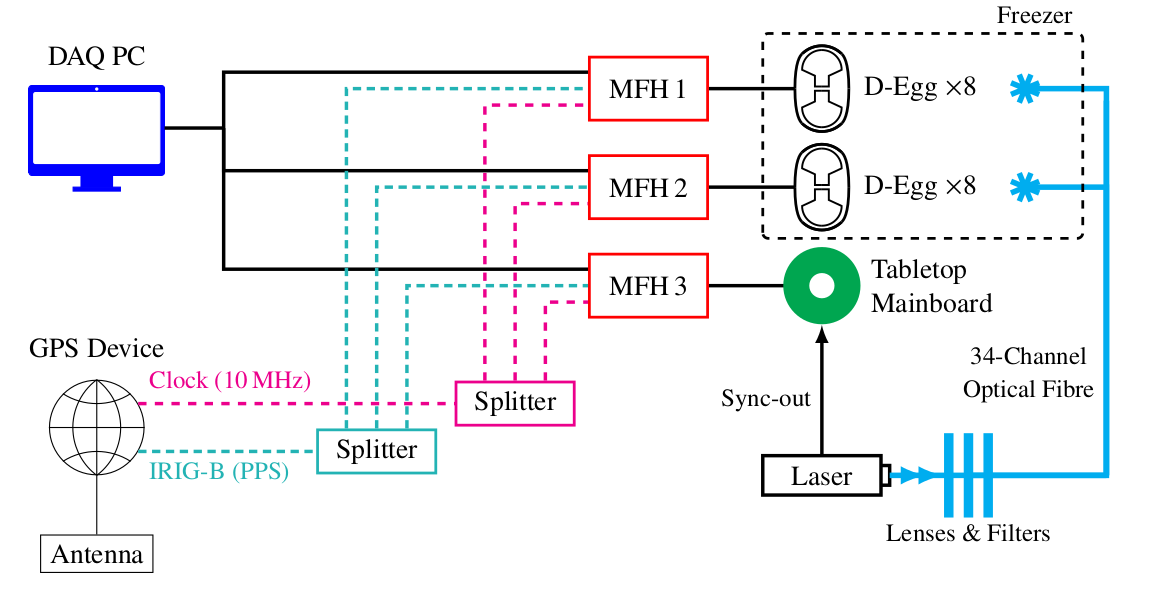
\includegraphics[width=\linewidth]{figures/fat_layout.png}
    \caption{A schematic layout of the FAT apparatus. }
    \label{fig:fatscheme}
\end{figure}

The block-diagram FAT facility and network architecture is shown in Figure~\ref{fig:fatscheme}. 
The DAQ PC is used to communicate with the D-Eggs via two Mini FieldHubs (MFHs); these are simplified versions of the hardware used on-site at the South Pole to communicate with in-ice DOMs. 
A third MFH is used to synchronize timing between a pulsed laser source and the other two MFHs: the Mini FieldHubs and DAQ PC are shown in Figure~\cite{fig:degg_fat_pc}.
The light source used to test the PMT response is a Hamamatsu PLP-10 C10196 with a 400 nm picosecond laser diode head M10306.
Two programmable filter wheels with six distinct neutral density filters are used to attenuate the laser light by discrete amounts. 
The laser light is carried through optical fiber and a series of splitters to expose both the top and bottom PMTs of each D-Egg; sixteen total PMTs.
This allows for the characterization of the gain of each D-Egg PMT at light levels ranging from low-occupancy SPE signals to levels greater than 200 SPE. 

\begin{figure}
    \centering
    \includegraphics[width=0.7\linewidth]{figures/degg/20221204232321_IMG_5392.JPG}
    \caption{Working on one of the Mini FieldHubs at the International Center for Hadron Astrophysics in Chiba, Japan; the DAQ PC can be seen running in the background.}\label{fig:degg_fat_pc}
\end{figure}

A 10 MHz clock and the IRIB-B GPS time signals are split and fed into each of the MFHs to synchronize their internal clocks to UTC.
This allows for conversion of the internal D-Egg timestamps to UTC using the standard IceCube Reciprocal Active Pulsing (RAPCal) method~\cite{ABBASI2009294}.

Data readouts for the PMTs are triggered in two ways: an Analog-to-Digital Converter (ADC) counts trigger, and a Finite Impulse Response (FIR) trigger. 
In the former, the analog current from the waveform is discretized into a time-dependent number of counts. 
Generally single-electron events are then used to calibrate the number of ADC counts to a physical quantity.
Then, a threshold number of ADC counts measured is used as a trigger to indicate when an event occurs in the PMT. 
FIR triggering, on the other hand, uses a rolling-average of the raw waveform before the ADC conversion happens. 
This smooths out the waveform and typically yields a lower dark rate.

%\subsection{Quick Monitoring}

\subsection{Detailed Monitoring}

As the temperature in the freezer is moving to its new target temperature, gain scans are regularly performed on the D-Eggs. 
The D-Egg PMTs have been independently measured to have an SPE pulse full-width half-maximum of approximately 14 nanoseconds and an amplitude of approximately 12 mV. 
Mainboard electronics on the D-Eggs broaden these pulses to an approximate amplitude of 6mV and FWHM of 20ns. 
As such, a trigger threshold of 2.0mV is typically used.

To calculate the gain, a charge distribution is first constructed from the read-out SPE waveforms by integrating from ten bins before the peak to fifteen bins after it.
A Gaussian is then fitted to the charge histogram, whose peak corresponds to the PMT voltage at a given set high-voltage. An example SPE waveform and charge distribution is shown in Figure~FIG.
This procedure is repeated at varying high voltages until the calculated gain is within $\pm 2\%$ of $10^{7}$.
A typical high voltage found is around 1500V. 

\subsection{Analyses}

Once the measurements are taken, data are transferred from the local DAQ PC to the grappa server system in Chiba. Several analyses are then performed, as described in Ref.~\cite{degg}. 
Tests are then ran on the results of these analyses, which are enumerated in Table~\ref{table:degg_tests}. 

\begin{table}
    \centering
    \rowcolors{2}{gray!25}{white}
    \begin{tabular}{c|cc}\rowcolor{blue!25}
        Quantity & Temperature & Criteria\\\hline
        HV at 1e7 Gain & Various & $1000\leq x \leq 2000$ \\
        darknoise max & Various & $x \leq 4000$ \\
        darknoise $\delta t$ & Various & $x \leq 3.5$ \\        
        timing resolution & Various & $x \leq 3.5$ \\
        $Q_{obs}/Q_{ideal}$ at 200pe & -20, -5 & $0.6\leq x$ \\
        $I_{obs}/I_{ideal}$ at 200pe & -20, -5 & $0.6\leq x$ \\
        double pulse separation & -20 & $x \leq 4000$ \\
        double pulse peak-to-valley & -20, -5 & $1.5\leq x\leq 2.0$ \\
        double pulse peak-to-valley 2 & -20, -5 & $1.75\leq x\leq 2.8$ \\
    \end{tabular}
    \caption{The tests ran}\label{table:degg_tests}
\end{table}

The most important of these is the gain analysis. 
We verify that each PMT is capable of reaching a gain of 1e7 at a high voltage between 1-2 kV. 
In addition to that, we verify a linear relationship exists between the high voltage and the log of the gain. 
An example of a good high-voltage versus gain relationship is shown in Figure~\ref{fig:degg_gain_curve}.

\begin{figure}
    \centering
    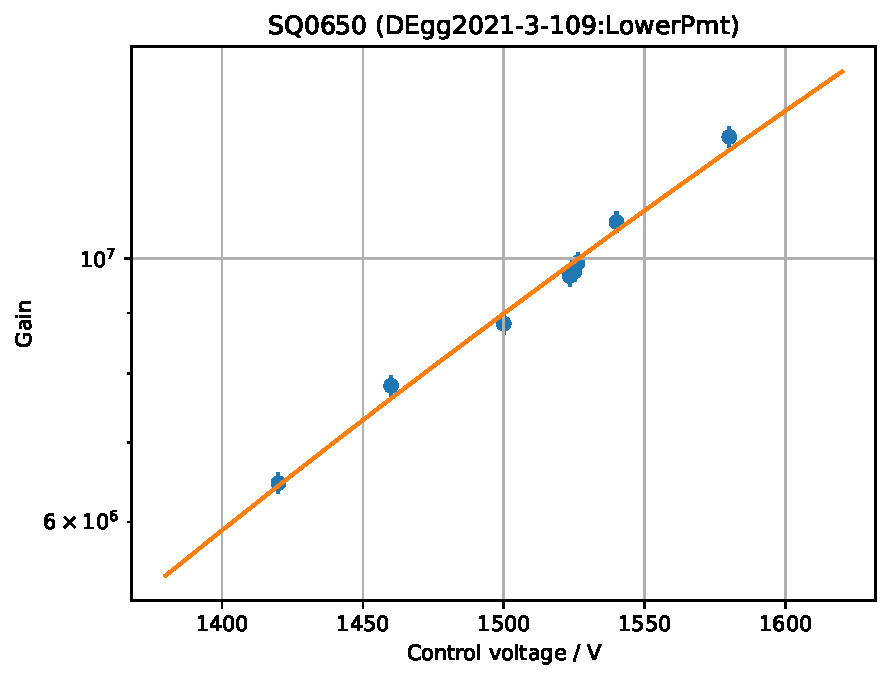
\includegraphics[width=0.8\linewidth]{figures/gain_curve_SQ0650.pdf}
    \caption{The gain fit for DEgg \texttt{DEgg2021-3-109}'s lower PMT, \texttt{SQ0650}. Data are shown in blue diamonds and the fit is shown in orange.}\label{fig:degg_gain_curve}
\end{figure}

Dark noise rates are also verified to be within acceptable bounds.
Dark noise describes any events that trigger the detector and which do not originate from an external photon hitting the detector. 
The sources of these photons are thermionic cathode emissions, PMT afterpulses, and any radioactive processes within the glass pressure vessel. 
These have been observed to be highly dependent on temperature. 

Two triggering methods are used; one uses a simple ADC triggering and the other uses the FIR-filtered triggering. Test are done for each D-Egg to verify that the dark noise rates do not ever exceed 10 MHz, and it should not consistently exceed 10kHz.
For the FIR-smoothed rates, we verify that the trigger rate does not exceed 5kHz. 
Figure~\ref{fig:dark_rate} shows examples of good and bad dark rates. 

\begin{figure}
    \centering
    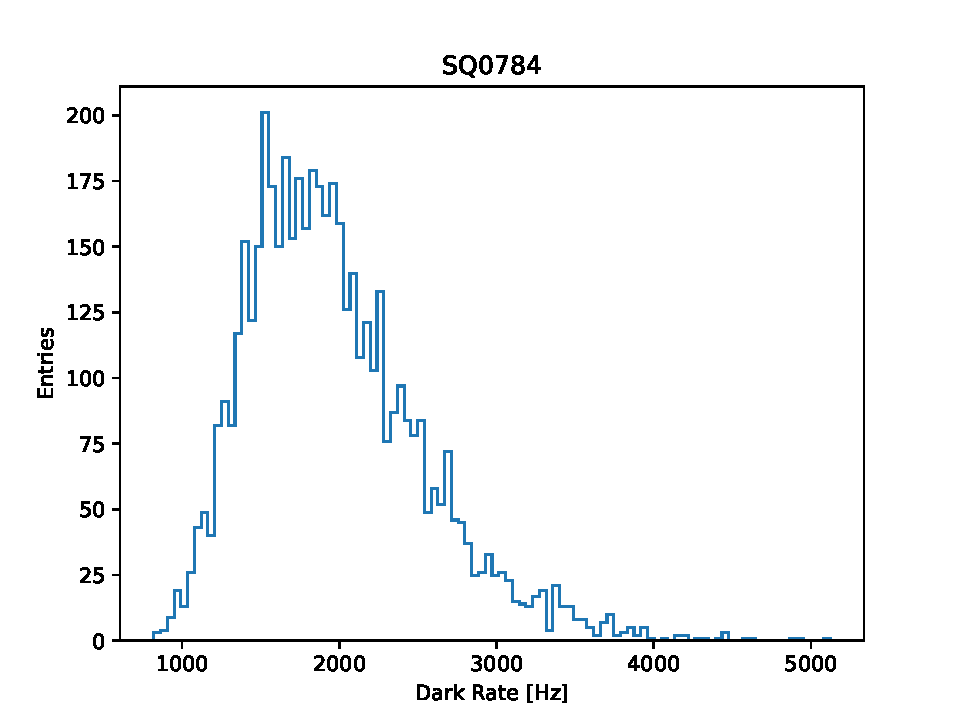
\includegraphics[width=0.45\linewidth]{./figures/dark_rate_SQ0784.pdf}%
    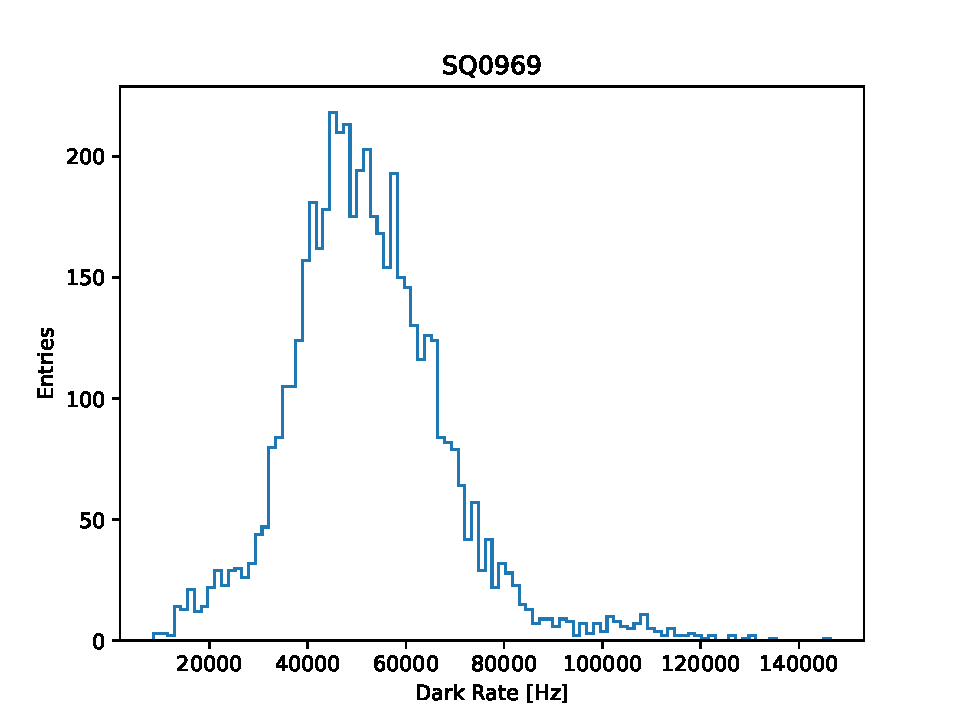
\includegraphics[width=0.45\linewidth]{./figures/dark_rate_SQ0969.pdf}
    \caption{Histograms showing the dark rates for PMTs \texttt{SQ0784} (left) and \texttt{SQ0969} (right). Dark rates are abnormally high for PMT \texttt{SQ0969}.}\label{fig:dark_rate}
\end{figure}

We also measure the linearity of the D-Egg response when compared to a known amount of injected light. 
By using the D-Egg filter wheels, the amount of light incident on the PMTs can be set to nine different settings ranging from 2.5\% to 100\%. 
The test laser intensity was also calibrated such that a 5\% filter corresponds to an observed signal of few 10s of PMTs. 

\begin{figure}
    \centering
    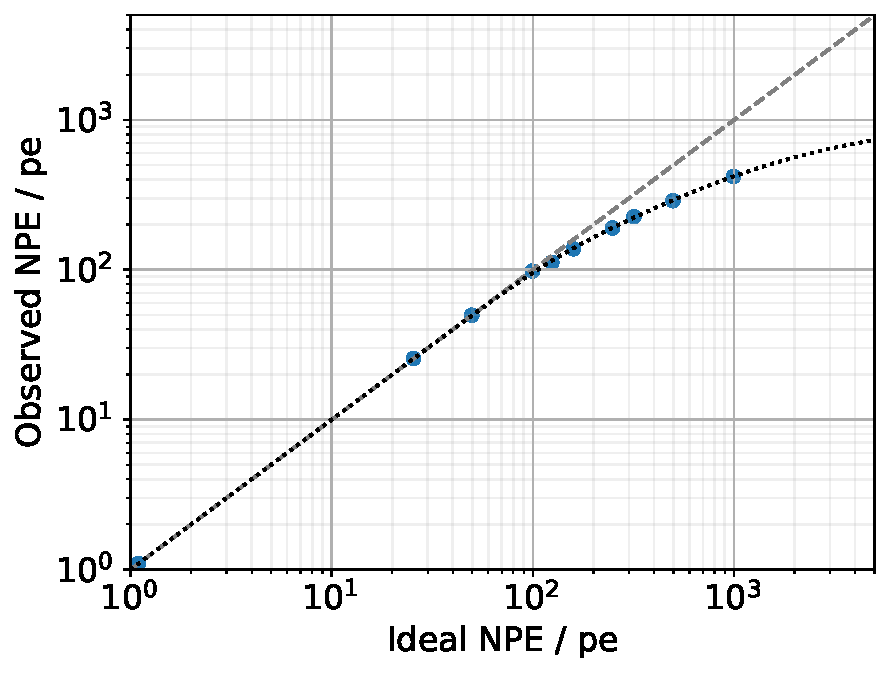
\includegraphics[width=0.7\linewidth]{figures/SQ0514_NPE_ideal_vs_observed.pdf}
    \caption{Linearity of the charge-response for PMT \texttt{SQ0514}. Measurements are shown as blue dots and a linear fit is shown as a dotted line. This is an example of a good linearity relationship.}
\end{figure}

One additional analysis is performed to test the ability of the D-Eggs to distinguish between the light from a charged tau lepton and its decay product. 
This requires being able to separately identifying two PMT pulses separated by only a few nano-seconds. 
To emulate a tau-like signal, a function generator creates two picosecond bursts separated by 20 nanoseconds. 
The generator creates then waits one microsecond before creating another burst of pulses. 
A peak-finding algorithm is then run 5000 digitized waveforms and the separation of the fit peaks are verified to be consistent with 20 nanoseconds and any error within half of the width mainboard timing bins.
An example good PMT response to this double-pulse test is shown in Figure~\ref{fig:double_pulse}.

\begin{figure}
    \centering
    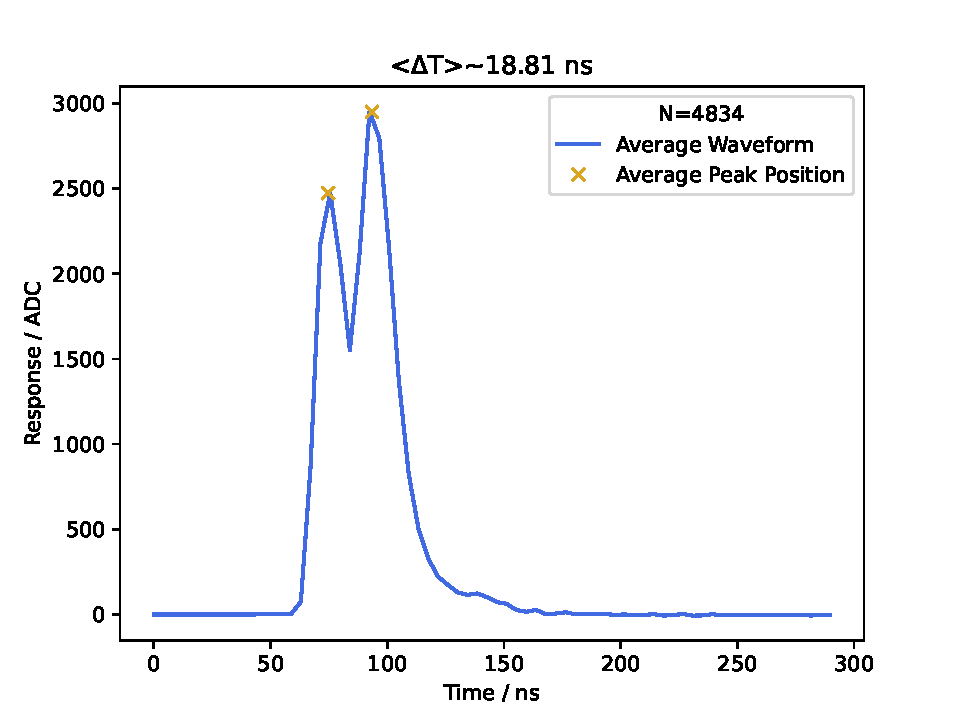
\includegraphics[width=0.8\linewidth]{figures/ave_wf_bl_sub_every_wf_DEgg2021-3-082_SQ1016.pdf}
    \caption{Averaged waveform of 5000 double-pulse signal tests for PMT \texttt{SQ1016}. A fit peak-separation of 18 nanoseconds; this is consistent with the injected 20 nanosecond signal separation to within half the width of the mainboard timing bins.}\label{fig:double_pulse}
\end{figure}

The results of all analyses and tests are automatically compiled into a pdf by software I developed and wrote.
A PDF for each D-Egg is generated including a table of the test results and relevant plots for failed tests are fetched and included. 
A second PDF is generated which summarizes the results of each D-Egg's tests and lists it as either Passing, Failing, or concerning. 
In the latter, it raises warning, and individual intervention is required to decide if the D-Egg will go to the pole or be left behind. 
An example D-Egg FAT result file is included in Appendix~\ref{append:degg_fat}.

\end{document}